%!TEX root = ../thesis.tex
%*******************************************************************************
%****************************** Third Chapter **********************************
%*******************************************************************************
\graphicspath{{Chapter3/Figs/Vector/}{Chapter3/Figs/}}

%%%%%%%%%%%%%%%%%%%%%%%%%%%%%%%%%%%%%%%%%%%%%%%%%%%%%%%%%%%%%%%%%%%%%%%%%%%%%%%%
% System Architecture
%%%%%%%%%%%%%%%%%%%%%%%%%%%%%%%%%%%%%%%%%%%%%%%%%%%%%%%%%%%%%%%%%%%%%%%%%%%%%%%%
% - What is most fitting solution to integrate TPS and UI into the
%   existing architecture?
%
\chapter{System Architecture}
\section{Introduction}
% Waar gaat dit hoofdstuk over?

% FRONTEND? BACKEND? PORTAL? TPS?
\mynote{verbeter intro door backend frontend te definieren}
The price calculation system that is being made should integrate in the existing architecture seamlessly. This chapter aims to answer question number two, and its subquestions. First it is determined whether the frontend and backend that are to be developed should be integrated in existing projects, or should be made in separate projects altogether. If the backend is created as a separate project, authentication and authorization are directly affected by these decisions. Separation implies more complex identity management, or less separation of concern. Then, the database should be capable of storing geometry, and accept queries to determine which polygons contain a set of points, and which points are contained within a polygon.

%%%%%%%%%%%%%%%%%%%%%%%%%%%%%%%%%%%%%%%%%%%%%%%%%%%%%%%%%%%%%%%%%%%%%%%%%%%%%%%%
% Architectural Patterns
%%%%%%%%%%%%%%%%%%%%%%%%%%%%%%%%%%%%%%%%%%%%%%%%%%%%%%%%%%%%%%%%%%%%%%%%%%%%%%%%
% - Which architectural patterns fit in with the exising architecture?
%
\section{Architectural Patterns}
The current system architecture consists of three public API's and eight private API's that connect to four databases, as can be seen in figure \ref{fig:Architecture}, and provide functionalities to portals and mobile apps.
The user interface, business logic, and data storage are separated, following the three-tier or multi-tier architecture \cite{IBM-3-tier}. Building the frontend and backend into one single project would be in conflict with this pattern, so the portal and TPS will be set up separately.

\begin{figure}[htbp!]
	\centering
	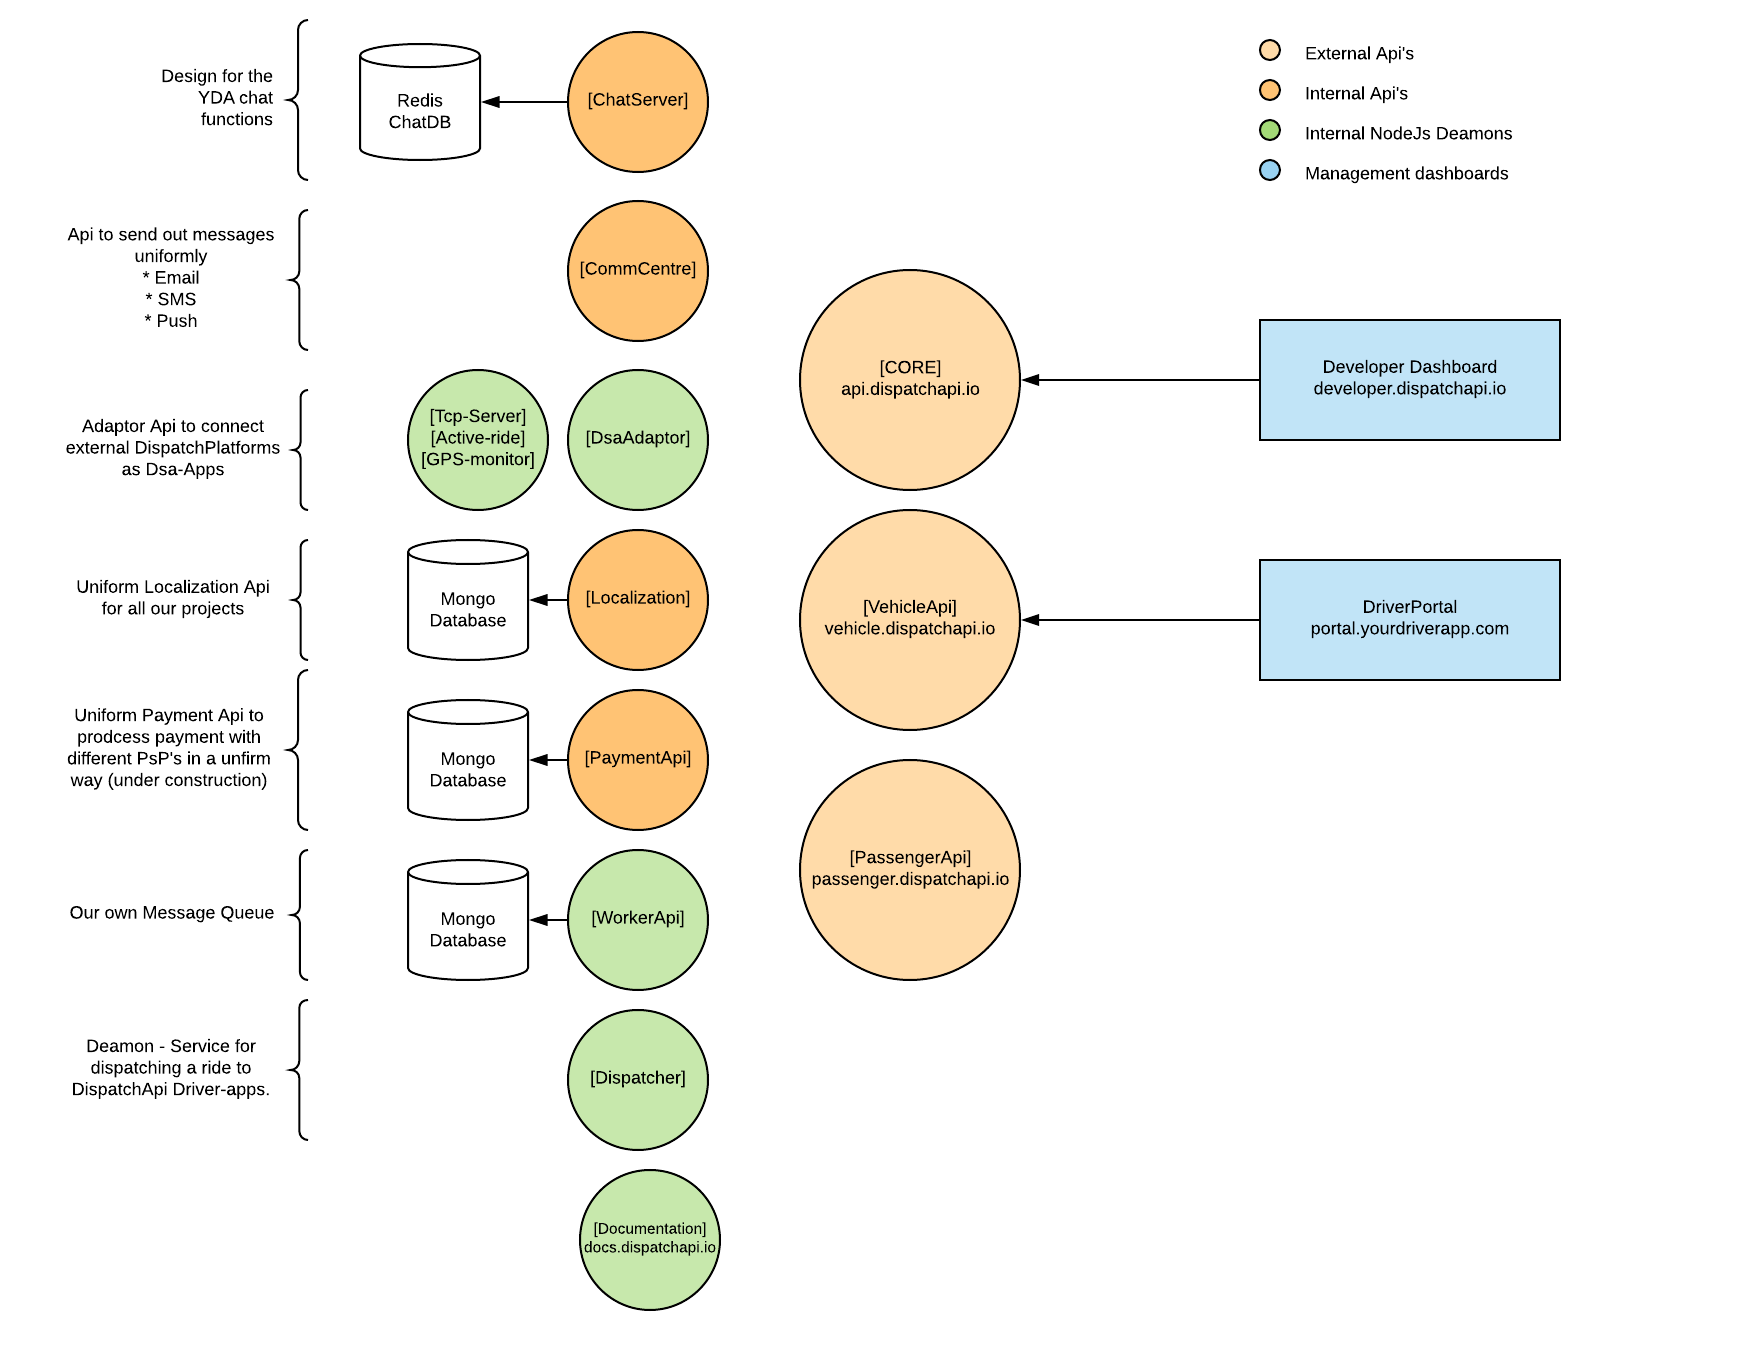
\includegraphics[width=1\textwidth]{Architecture}
	\caption[Architecture]{Current System Architecture}
	\label{fig:Architecture}
\end{figure}

% The option remains to integrate TPS and portal into the core API and YDA portal respectively.


Another pattern that is used is the service-oriented architecture, where application components provide services over a network typically.

It is possible to integrate the pricing system as a module in this existing project, simplifying authentication and authorization, because information is shared internally. Another option is to implement the system as a microservice, a service-oriented architecture (SOA), having the duty of offer a service to other components over the network.


Each microservice is responsible for managing and containing state to enable users who would like to use the system to be authenticated and authorized. Advantages of a microservice are the fact that a microservice is a self-contained and naturally modular structure, but authentication and authorization must be handled by the microservice itself, unless state is shared amongst services, which would eliminate the reason to use a microservice at all. In the present architecture, different services implement different authentication methods, store different information about different users. Authorization is managed by sending extra headers for each crucial piece of information. For example: company information, application information and user information are all sent in separate headers.


When the amount of services that are added to the architecture increases, the mount of information that is no longer centralized increases as well.


%%%%%%%%%%%%%%%%%%%%%%%%%%%%%%%%%%%%%%%%%%%%%%%%%%%%%%%%%%%%%%%%%%%%%%%%%%%%%%%%
% Accessing Necessary Data
%%%%%%%%%%%%%%%%%%%%%%%%%%%%%%%%%%%%%%%%%%%%%%%%%%%%%%%%%%%%%%%%%%%%%%%%%%%%%%%%
% - Which data is required to make TPS operational?
%
\section{Sharing Necessary Data}

\begin{itemize}
	\item User data
	\item Vehicle data
	\item etc..
\end{itemize}

%%%%%%%%%%%%%%%%%%%%%%%%%%%%%%%%%%%%%%%%%%%%%%%%%%%%%%%%%%%%%%%%%%%%%%%%%%%%%%%%
% Authentication and Authorization
%%%%%%%%%%%%%%%%%%%%%%%%%%%%%%%%%%%%%%%%%%%%%%%%%%%%%%%%%%%%%%%%%%%%%%%%%%%%%%%%
% - How can authentication between services be implemented or improved?
%
\section{Authentication and Authorization}
Mobile applications should be able to make requests, just like the portals that are to be developed. But portal users make use of the microservice in a different way. Mobile apps merely request prices of products, based on the rules that group admins define through the portal. To make sure that only the portal users have the right to mutate their data, users have to be authenticated and authorized within the microservice. Identity management becomes a problem if data duplication is not desired. If a user makes a direct request to the microservice, the credentials have to be compared to user data in a database. To prevent duplication, the microservice could be connected to the database that is used by the core system. But this makes the microservice less decoupled, and directly contradicts the desire to separate concerns. Four examples demonstrate this problem:

\begin{itemize}
	\item Example 1: The microservice authenticates and authorizes users all by itself, managing sessions and storing user data in its database.
	\item Example 2: The microservice connects to an exising databases to acquire the required information about the user.
	\item Example 3: The core system authenticates the user and provides a token that can be verified by the microservice, containing user identity.
	\item Example 4: A separate service is used for authentication and authorization so that the core system is not involved at all.
\end{itemize}

In the first example, the microservice seems to work independently, because it has knowledge about the users identity without making requests to adjecent systems, or connecting to external databases. But this is not true. If data about the user is mutated in the core system, the microservice needs to be notified or synced. This greatly hinders scaling and makes it harder to keep data consistent. Example two solves the inconsistency part by connecting to the central database that holds user data, but contradicts the strive for encapsulation.

\subsection{JSON Web Tokens}
Example three entirely removes the database connection to any user data. This is possible when a JSON Web Token (JWT) is used. A JWT may be signed with a cryptographic algorithm or even a public/private key pair using RSA. After the user enters valid credentials, the core system validates the credentials by comparing them with user data in the database. The core system signs a token that with a secret that is known by the microservice. The token consists of three parts, separated by a fullstop. The first part (header) of the token contains information about the hashing algorithm that was used to encrypt the payload. This part is Base64Url encoded. The payload itself contains information stored in JSON format:

\mynote{Show diagram with hierarchy of companies and apps}

\begin{center}
	\begin{tikzpicture}
		\draw  (-2,5) rectangle (1,3);
	\end{tikzpicture}
\end{center}

\mynote{Make }

\begin{Verbatim}[fontsize=\scriptsize]
	{
		"companyId": "59ea0846f1fea03858e16311",
		"daAppInstallId": "599d39b67c4cae5f11475e93",
		"iat": 1521729818,
		"exp": 1521816218,
		"aud": "tps.dispatchapi.io",
		"iss": "api.dispatchapi.io",
		"sub": "getPrices"
	}
\end{Verbatim}

The identity of the user is stored in the payload that can only be revealed by whoever holds the secret with which it was signed. Then the message can be verified using the third part of the token, which is the signature. This verification step prevents tampering with the payload.

\subsection{oAuth 2.0}
Example four delegates managing user identity to a separate authentication service that, similar to the pricing microservice, has its own single task of authenticating users. OAuth 2.0 is a protocol that has been designed to allow third-party apps to grant access to an HTTP service on behalf of the resource owner. This behaviour could be utilized to allow users to make use of services within the architecture, controlled by a single service, stored in a single token. A proposal was made in the Pregame document to combine oAuth with JWT and an API Gateway to introduce an automated authentication flow with a single token, instead of sending multiple headers, see Appendix \ref{appendix:pregame}.

\begin{figure}[ht!]
	\centering
	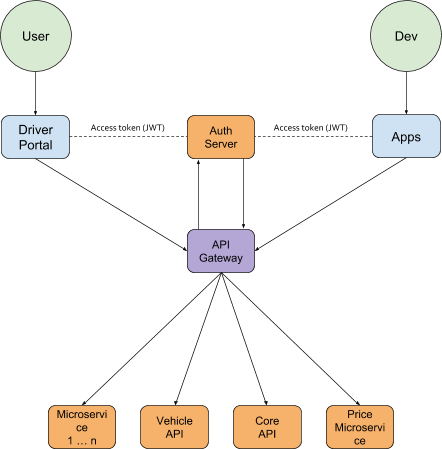
\includegraphics[width=.7\textwidth]{OAuth}
	\caption[Architecture]{oAuth, API Gateaway, using JWT}
	\label{fig:oAuth}
\end{figure}
\clearpage

\subsection{API Gateway}

Another common structure that allows services to be used by external agents is the API Gateway. It allows for a central middleware in which authentication and authorization is handled, where the microservices are shielded from public access, and all communication is established through the API Gateway [4].

Next to authentication, the gateway could optimize the endpoints so that no multiple requests are needed from external agents to gather different types of resources. These calls could be made internally to the microservices behind the gateway. This also opens the possibility the freely change the microservices without changing the public endpoints exposed by the gateway, and even offers slow or instant transitions to different versions of microservices.

The different proposals explain the improvements they may bring over some system. But the advice given is not tied to this project, instead to the entire Dispatch API. It’s advised to have a constructive dialogue about the future of the company, and the way it’s planning to scale. One could put a API Gateway in front of a monolithic app to help with transitioning to a microservice-oriented app.

%%%%%%%%%%%%%%%%%%%%%%%%%%%%%%%%%%%%%%%%%%%%%%%%%%%%%%%%%%%%%%%%%%%%%%%%%%%%%%%%
% Authentication and Authorization
%%%%%%%%%%%%%%%%%%%%%%%%%%%%%%%%%%%%%%%%%%%%%%%%%%%%%%%%%%%%%%%%%%%%%%%%%%%%%%%%
% - Which methods and technologies can be used to ensure suitability and
%   improve maintainability and testability?
%
\section{Suitability of Methods and Technologies}
\mynote{Write chapter about methods and technologies}
\begin{itemize}
	\item Node JS, PHP, MongoDB, MySQL, Microservice, Loopback, Graph QL,
	\item Slides and proposals
	\item Mocha, Buddy-Works, Circle CI, Typescript, Chai, Functional Programming
\end{itemize}
